\subsection{Speed analysis}
In this section, we investigate the average speed $\overline{speed}$ in each status. For example, taxi i drives in occupied status for a distance $d$ using time $t$, then the average speed in this status is $d/t$.
From March 3th to 7th, 2011, the $\overline{\overline{speed}_{empty}} = 3.627 m/s$, while that for occupied status is $\overline{\overline{speed}_{occupied}}=7.083 m/s$.

\begin{figure}[!h]
\centering
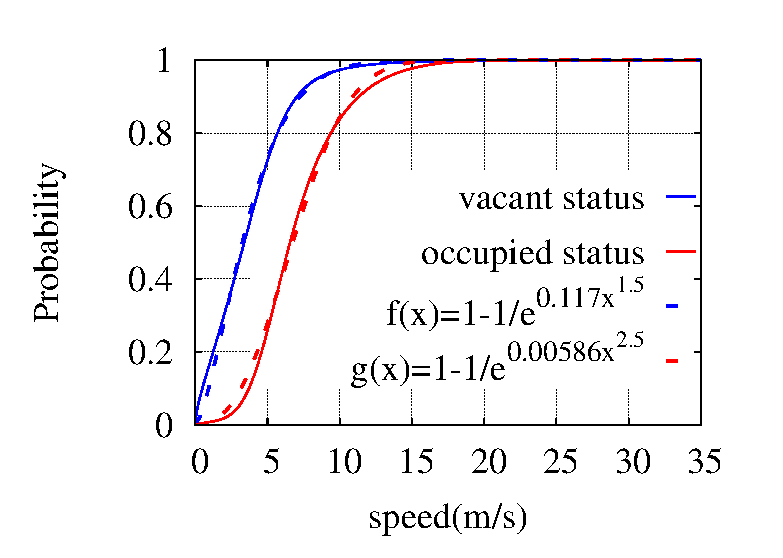
\includegraphics[width=0.3\textwidth]{figures_201103/fit/speedfit.eps}
\caption{$\overline{speed}$ distribution for vacant and occupied statuses.}\label{figure_speed_distribution}
\end{figure}

To further investigate the cumulative speed distribution, proportion for every $\overline{speed}$ section is calculated.
As shown in Fig.\ref{figure_speed_distribution}. For example, dot(20,0.0245) means $2.45\%$ records fall in the range $[0,20)km/h$. We also fit the speed to model the microscope behavior, which will be shown in section \ref{section_modeling}
Fig. \ref{figure_speed_distribution} shows that $\overline{speed}$ distribution differs for each status. For vacant status, the $\overline{speed}$ gather together at  \ref{figure_speed_distribution} also demonstrates that the speed distribution is with strong regularity for each status.


